\documentclass[10pt,a4paper]{scrartcl}
\usepackage[utf8]{inputenc}
\usepackage{amsmath}
\usepackage{amsfonts}
\usepackage{amssymb}
\usepackage{tikz}
\usepackage{mathpazo}
\usetikzlibrary{patterns}
\usepackage[a4paper,
left=3.0cm, right=3.0cm,
top=2.0cm, bottom=2.0cm]{geometry}
\usepackage{fullpage}
\usepackage[german]{babel}
\usepackage{pst-all}
\usepackage{pstricks}
\usepackage{floatflt}
\usepackage{listings}
\usepackage{courier}
 \lstset{
         basicstyle=\footnotesize\ttfamily, % Standardschrift
         %numbers=left,               % Ort der Zeilennummern
         numberstyle=\tiny,          % Stil der Zeilennummern
         %stepnumber=2,               % Abstand zwischen den Zeilennummern
         numbersep=5pt,              % Abstand der Nummern zum Text
         tabsize=2,                  % Groesse von Tabs
         extendedchars=true,         %
         breaklines=true,            % Zeilen werden Umgebrochen
         keywordstyle=\color{red},
    		frame=b,         
 %        keywordstyle=[1]\textbf,    % Stil der Keywords
 %        keywordstyle=[2]\textbf,    %
 %        keywordstyle=[3]\textbf,    %
 %        keywordstyle=[4]\textbf,   \sqrt{\sqrt{}} %
         stringstyle=\color{white}\ttfamily, % Farbe der String
         showspaces=false,           % Leerzeichen anzeigen ?
         showtabs=false,             % Tabs anzeigen ?
         xleftmargin=17pt,
         framexleftmargin=17pt,
         framexrightmargin=5pt,
         framexbottommargin=4pt,
         %backgroundcolor=\color{lightgray},
         showstringspaces=false      % Leerzeichen in Strings anzeigen ?        
 }
 \usepackage{caption}
\DeclareCaptionFont{white}{\color{white}}
\DeclareCaptionFormat{listing}{\colorbox[cmyk]{0.43, 0.35, 0.35,0.01}{\parbox{\textwidth}{\hspace{15pt}#1#2#3}}}
\captionsetup[lstlisting]{format=listing,labelfont=white,textfont=white, singlelinecheck=false, margin=0pt, font={bf,footnotesize}}

\usepackage{color}
\usepackage{enumerate}
\setlength{\unitlength}{1cm}
\newcommand{\N}{\mathbb{N}}
\newcommand{\A}{\mathcal{A}}
\newcommand{\R}{\mathbb{R}}
\author{Tom}
\title{Analysis 2 - Hausaufgabe 2}
\begin{document}
\begin{center}
\textsc{\Large{Analysis 2 - Hausaufgabe 2}} \\
\end{center}
\begin{tabbing}
Tom Nick \hspace{1.4cm}\= 342225\\
Tom Lehmann\>  340621\\
Maximilian Bachl\> 123456
\end{tabbing}
\subsection*{Aufgabe 1.}
\begin{enumerate}[(i)]
\item
\begin{minipage}{0.49\columnwidth}
\begin{lstlisting}[caption= Mathematica Code für die Niveaulinien von h]
ContourPlot[{x^2/4 + y^2/9 + 4 == 4, 
x^2/4 + y^2/9 + 4 ==  5, 
x^2/4 + y^2/9 + 4 == 8}, 
{x, -6, 6}, {y, -6, 6},
ContourStyle -> Black]
\end{lstlisting}
Eine allgemeine Vorschrift für Niveaulinien zum Wert $c$ ist: $\frac{x^2}{4} + \frac{y^2}{9} + 4 =c$ bzw. nach $y$ umgestellt: $$y = \sqrt{9c + 36 + \frac{9x^2}{4}}$$
\end{minipage}
\begin{minipage}{0.49\columnwidth}
$\qquad$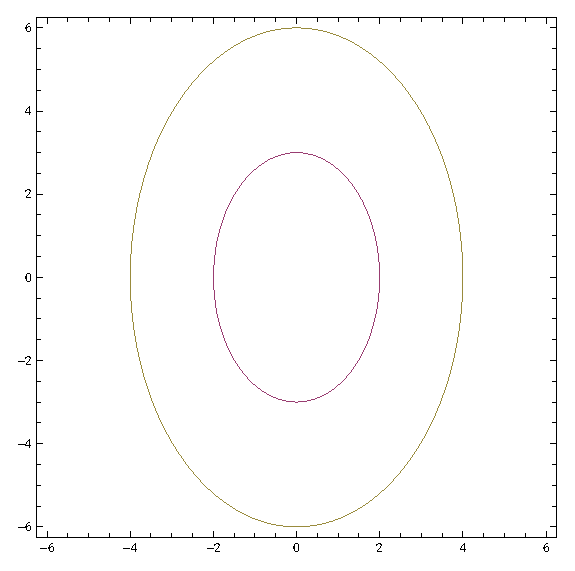
\includegraphics[scale=0.7]{1i.eps} 
\end{minipage}
\item 
\begin{minipage}{0.50\columnwidth}
\begin{lstlisting}[caption= Mathematica Code für den Graph von h]
Plot3D[x^2/4 + y^2/9 + 4, 
{x, -6, 6}, {y, -6, 6},
PlotStyle -> None]
\end{lstlisting}
\end{minipage}
\begin{minipage}{0.50\columnwidth}
$\qquad$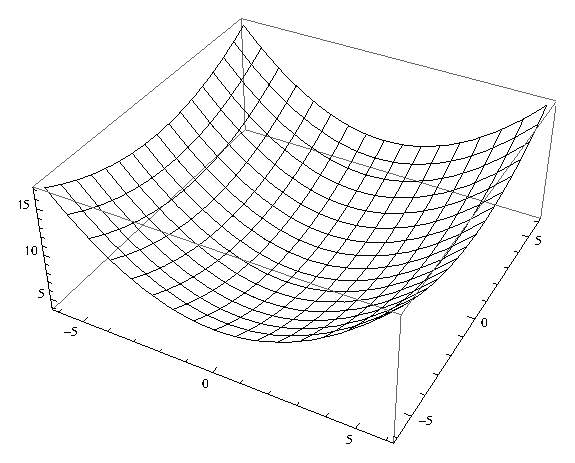
\includegraphics[scale=0.7]{1ii.eps} 
\end{minipage}
\item 
+Da $f$ eine Komposition von stetigen Funktionen ist, sowie das Intervall $D$ kompakt ist, muss $f$ Minima und Maxima in $D$ annehmen. Anhand der Bilder ist ein leichtes zu sehen, wo Minima und Maxima auftreten. \textbf{Minima: } $f(0,0) = 4$, \textbf{Maxima: } %$f(0,1) = \frac{52}{9}$
$f(-2,0) = 5 = f(2,0)$
\item 
Man kann $\vec{Z}$ nicht zeichnen, da man 6 Dimensionen nicht darstellen kann.  \\
\begin{minipage}{0.49\columnwidth}
Wählt man jedoch $r=1$ sieht das ganze so aus:
\begin{lstlisting}[caption= Mathematica Code für den Graph von Z]
ParametricPlot3D[{Cos[phi], Sin[phi], z}, 
{phi, 0, 2 \[Pi]}, {z, 0, 2}, 
PlotStyle -> None, BoundaryStyle -> Black]
\end{lstlisting}
\end{minipage}
\begin{minipage}{0.50\columnwidth}
$\qquad$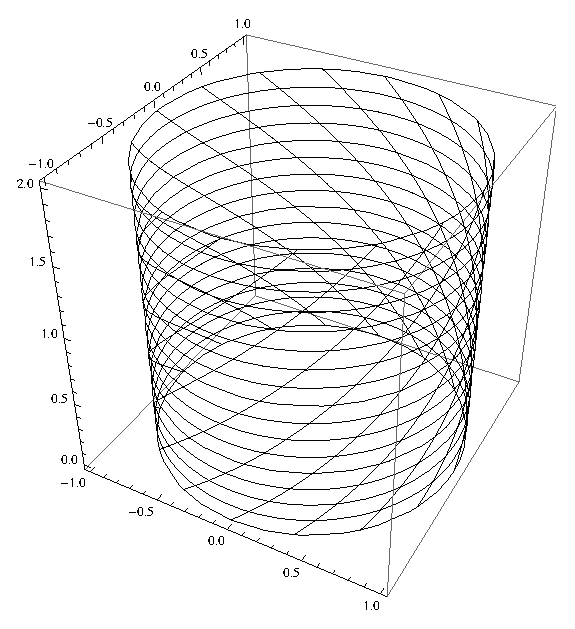
\includegraphics[scale=0.7]{1iv.eps} 
\end{minipage}
\begin{minipage}{0.50\columnwidth}
Wählt man $z = 1$, aber lässt $r$ variabel:
\begin{lstlisting}[caption= Mathematica Code für den Graph von Z]
ParametricPlot3D[{r*Cos[t], r*Sin[t], 1}, 
{t, 0, 2 \[Pi]}, {r, 0, 1}, 
PlotStyle -> None, BoundaryStyle -> Black]
\end{lstlisting}
\end{minipage}
\begin{minipage}{0.50\columnwidth}
$\qquad$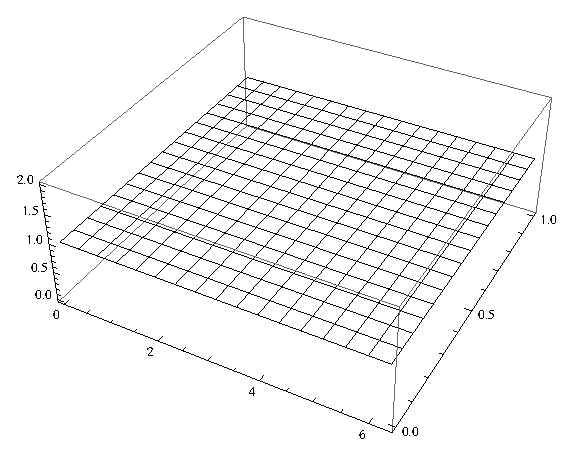
\includegraphics[scale=0.7]{1iv2.eps} 
\end{minipage}
\end{enumerate}
\subsection*{Aufgabe 2.}
$f$ ist an den Punkten $(x,y) \neq (0,0)$ stetig da, $\frac{x^2y^2+y^8}{x^2+y^4}$ eine Komposition stetiger Funktionen ist. Sei die Stetigkeit am Punkt $(x,y) = (0,0)$ zu überprüfen.
\begin{align*}
\lim_{\vec{x} \to \vec{0}} \left| f(x,y) - f(0,0) \right| &= \lim_{\vec{x} \to \vec{0}} \left| \frac{x^2y^2+y^8}{x^2+y^4} - 0 \right| \\
 &= \lim_{\vec{x} \to \vec{0}} \left| \frac{x^2y^2+y^8}{x^2+y^4}\right| \\
 &\geq \lim_{\vec{x} \to \vec{0}} \left| \frac{x^2y^4+y^8}{x^2+y^4}\right| \\
 &= \lim_{\vec{x} \to \vec{0}} \left| \frac{(x^2+y^4)y^4}{x^2+y^4}\right| \\
 &=  \lim_{\vec{x} \to \vec{0}} \left| y^4 \right| \\
 &= 0
\end{align*}
Damit ist $f$ auch im Punkt $(0,0)$ stetig, womit sie stetig auf $\R^2$ ist. \\

$g$ ist an den Punkten $(x,y) \neq (0,1)$ stetig da, $\frac{x^4(y-1)^2+x^3(y-1)^3}{(x^2+(y-1)^2)^3}$ eine Komposition stetiger Funktionen ist. Sei die Stetigkeit am Punkt $(x,y) = (0,1)$ zu überprüfen.
%\begin{align*}
%\lim_{\vec{x} \to \vec{0}} \left| f(x,y) - f(0,0) \right| &= \lim_{\vec{x} \to \vec{0}} \left| \frac{x^2y^2+y^8}{x^2+y^4} - 0 \right| \\
% &= \lim_{\vec{x} \to \vec{0}} \left| \frac{x^2y^2+y^8}{x^2+y^4}\right| \\
% &\geq \lim_{\vec{x} \to \vec{0}} \left| \frac{x^2y^4+y^8}{x^2+y^4}\right| \\
% &= \lim_{\vec{x} \to \vec{0}} \left| \frac{(x^2+y^4)y^4}{x^2+y^4}\right| \\
% &=  \lim_{\vec{x} \to \vec{0}} \left| y^4 \right| \\
% &= 0
%\end{align*}
Damit ist $g$ im Punkt $(0,1)$ nicht stetig, womit die Funktion stetig auf $\R^2 \backslash \{ (0,1)\}$ ist. \\
\end{document}
